%!TEX encoding = UTF-8 Unicode
%!TEX root = ../lect-w06.tex

%%%

\ifkompendium\else
\Subsection{Veckans uppgifter}

\begin{SlideExtra}{Veckans övning: \texttt{patterns}}
  Mål: Träna på matchning (och undantag)
\begin{itemize}\SlideFontSmall
\item Uppg. 1--7: Matchning, \code{Option}
\item Uppg. 8--10: Undantag, \code{Try}
\item Fördjupn. 11: Matchning eller dynamisk bindning?
\item Fördjupn. 12: avgöra likhet med matchning, \code{equals} utan arv
\item Fördjupn. 13--23: diverse fördjupningsuppgifter om matchning, undantag, hash-koder, likhet vid arvshierarki
\end{itemize}
\end{SlideExtra}


\begin{SlideExtra}{Lab \texttt{blockbattle} läsvecka 5--6}
  \begin{minipage}{0.42\textwidth}
        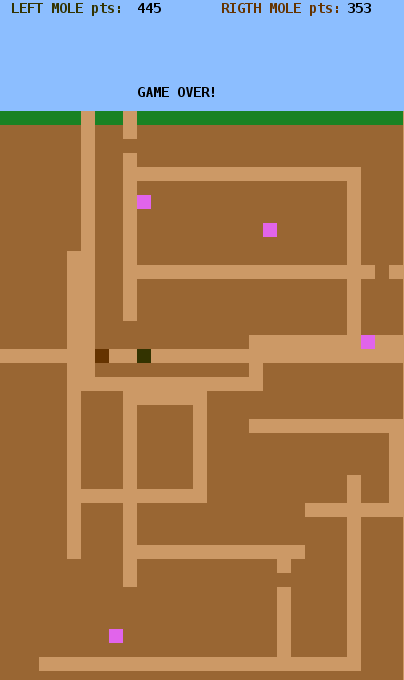
\includegraphics[height=0.8\textheight]{../img/blockbattle.png}
  \end{minipage}%
  \begin{minipage}{0.59\textwidth}
    \SlideFontSmall Tips på hur du kan träna på att använda mönstermatchning:
    \begin{itemize}\SlideFontSmall
      \item Händelsehantering med \code{match} i stället för nästlade \code{if}
      \item Ändra så att \code{waitForKeyNonBlocking} returnerar \code{Option[String]}
      \item Låt metoderna \code{setBlock} och \code{getBlock} genererar undantag om position är utanför fönstret. Använd \code{require} för att åstadkomma detta. 
      \item Använd \code{Try} när du anropar metoder som kan ge undantag och undvik att din app kraschar, men ge bra felmeddelande som underlättar avlusning.
    \end{itemize}    
  \end{minipage}
\end{SlideExtra}


% \begin{SlideExtra}{Specialundervisning}
% \begin{itemize}
% \item  \Alert{Specialundervisning} organiseras för de som har det extra svårt med grunderna och inte kommit igång med självständigt kodande.
% \item Specialundervisningen sker på dessa speciellt utvalda resurstider efter anmälning via enkät: \\ \Emph{Ons 15-17 E:Alfa} eller \Alert{Tor 13-15 E:Beta}. \\ Gruppindelning meddelades via mejl.  
% \item Du som \Alert{inte} deltar i specialundervisningen hänvisas till \Alert{rummet bredvid}, där \Emph{''vanlig''} resurstid pågår. 
% \end{itemize}
% \end{SlideExtra}


\fi

